\usetikzlibrary{calc,decorations.pathmorphing,arrows.meta}
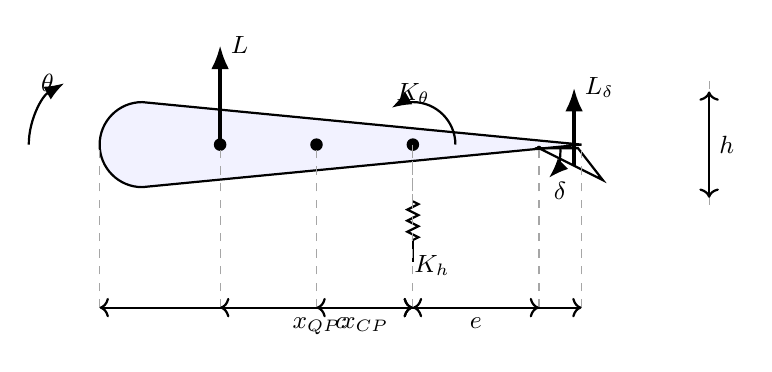
\begin{tikzpicture}[scale=0.9]
  \tikzset{
    foil/.style={thick, draw=black, fill=blue!5!white},
    point/.style={circle, fill=black, inner sep=1.6pt},
    force/.style={-{Latex[length=3mm]}, very thick},
    rotarrow/.style={-{Latex[length=2.5mm]}, thick},
    spring/.style={thick, decorate, decoration={zigzag, segment length=4pt, amplitude=2pt}},
    dashedline/.style={dashed, gray!70},
    dimarrow/.style={<->, thick},
    label/.style={font=\small}
  }

  % Chordwise coordinates reused from the original body diagram
  \coordinate (LE) at (0.2,0);
  \coordinate (TE) at (7,0);
  \coordinate (BottomMid) at (0.8,-0.6);

  \coordinate (Q) at ($(LE)!0.25!(TE)$);
  \coordinate (C) at ($(LE)!0.45!(TE)$);
  \coordinate (P) at ($(LE)!0.65!(TE)$);

  % Aileron hinge and tip (small deflected surface)
  \coordinate (Hinge) at ($(TE)+(-0.6,-0.05)$);
  \coordinate (AileronTip) at ($(Hinge)+(0.9,-0.45)$);

  % Draw original airfoil shape
  \draw[foil] (TE) -- (BottomMid) arc (270:90:0.6) -- cycle;

  % Draw aileron
  \draw[thick] (Hinge) -- ($(Hinge)+(0.55,0)$) -- (AileronTip) -- cycle;
  \fill (Hinge) circle (1pt);

  % Mark important points
  \node[point, label=above right:$Q$] at (Q) {};
  \node[point, label=above right:$C$] at (C) {};
  \node[point, label=above:$P$] at (P) {};

  % Lift forces
  \draw[force] (Q) -- ++(0,1.4) node[right, label] {$L$};
  \draw[force] ($(Hinge)!0.55!(AileronTip)$) -- ++(0,1.1) node[right, label] {$L_\delta$};

  % Pitch spring/damper moment at P
  \draw[rotarrow] ($(P)+(0.6,0)$) arc (0:120:0.6) node[above right=-2pt, label] {$K_\theta$};

  % Plunge spring under P
  \draw[dashedline] (P) -- ++(0,-0.8);
  \draw[spring] ($(P)+(0,-0.8)$) -- ++(0,-0.55);
  \draw[thick] ($(P)+(0,-1.35)$) -- ++(0,-0.3);
  \node[label, below right=-3pt] at ($(P)+(0,-1.55)$) {$K_h$};

  % Aileron deflection delta arrow
  \draw[rotarrow] ($(Hinge)+(0.3,0.02)$) arc (5:-45:0.55) node[below right=-2pt, label] {$\delta$};

  % Pitch angle theta arrow near leading edge
  \draw[rotarrow] ($(LE)+(-1.0,0)$) arc (180:120:1.0) node[left, label] {$\theta$};

  % Plunge displacement h indicator
  \draw[dashedline] ($(TE)+(1.8,0.9)$) -- ($(TE)+(1.8,-0.9)$);
  \draw[dimarrow] ($(TE)+(1.8,0.75)$) -- node[right, label] {$h$} ($(TE)+(1.8,-0.75)$);

  % Baseline for offsets
  \coordinate (BaselineY) at (0,-2.3);
  \draw[dashedline] (LE |- BaselineY) -- (LE);
  \draw[dashedline] (Q |- BaselineY) -- (Q);
  \draw[dashedline] (C |- BaselineY) -- (C);
  \draw[dashedline] (P |- BaselineY) -- (P);
  \draw[dashedline] (Hinge |- BaselineY) -- (Hinge);
  \draw[dashedline] (TE |- BaselineY) -- (TE);

  \draw[dimarrow] (LE |- BaselineY) -- node[below, label] {$c$} (TE |- BaselineY);
  \draw[dimarrow] (Q |- BaselineY) -- node[below, label] {$x_{QP}$} (P |- BaselineY);
  \draw[dimarrow] (C |- BaselineY) -- node[below, label] {$x_{CP}$} (P |- BaselineY);
  \draw[dimarrow] (P |- BaselineY) -- node[below, label] {$e$} (Hinge |- BaselineY);
\end{tikzpicture}
